\documentclass{beamer}

\input{../ts-glærur}

\title{FOR3R - meira um tímaflækjur}

\begin{document}

\section{Mælingar}

\begin{frame}
\titlepage
\end{frame}

\begin{frame}
\begin{itemize}
 \item Við höfum nokkra tímaflækjuflokka
 \begin{itemize}
  \item $\Theta(n)$, $\Theta(n^2)$, $\Theta(\sqrt{n})$, \ldots
 \end{itemize}
 \item En hvað þýðir þetta í alvörunni?
\end{itemize}
\end{frame}

\begin{frame}[fragile]{Dæmi: Viðsnúningur strengs}
Skoðum (lélegt) fall sem snýr við streng:

\inputminted{python}{Code/Python/slow_reverse.py}

Við sjáum eina lykkju, við getum \emph{giskað} á að tímaflækjan sé $O(n)$.
\end{frame}

\begin{frame}{Prófanir}
Prófa að keyra fallið \texttt{slow\_reverse}:
\begin{center}
\begin{tabular}{ll}
\toprule
$n$&$t_n$ (sek)\\
\midrule
100&0.072868\\
500&0.332766\\
1000&0.662849\\
10000&6.661191\\
\bottomrule
\end{tabular}
\end{center}
Hér er $n$ lengd strengsins \texttt{str} sem snúið er við, og $t_n$ tíminn sem tók að keyra \texttt{slow\_reverse(str)} $1000$ sinnum.
\end{frame}

\begin{frame}{Niðurstöður prófana - bein lína}
\begin{center}
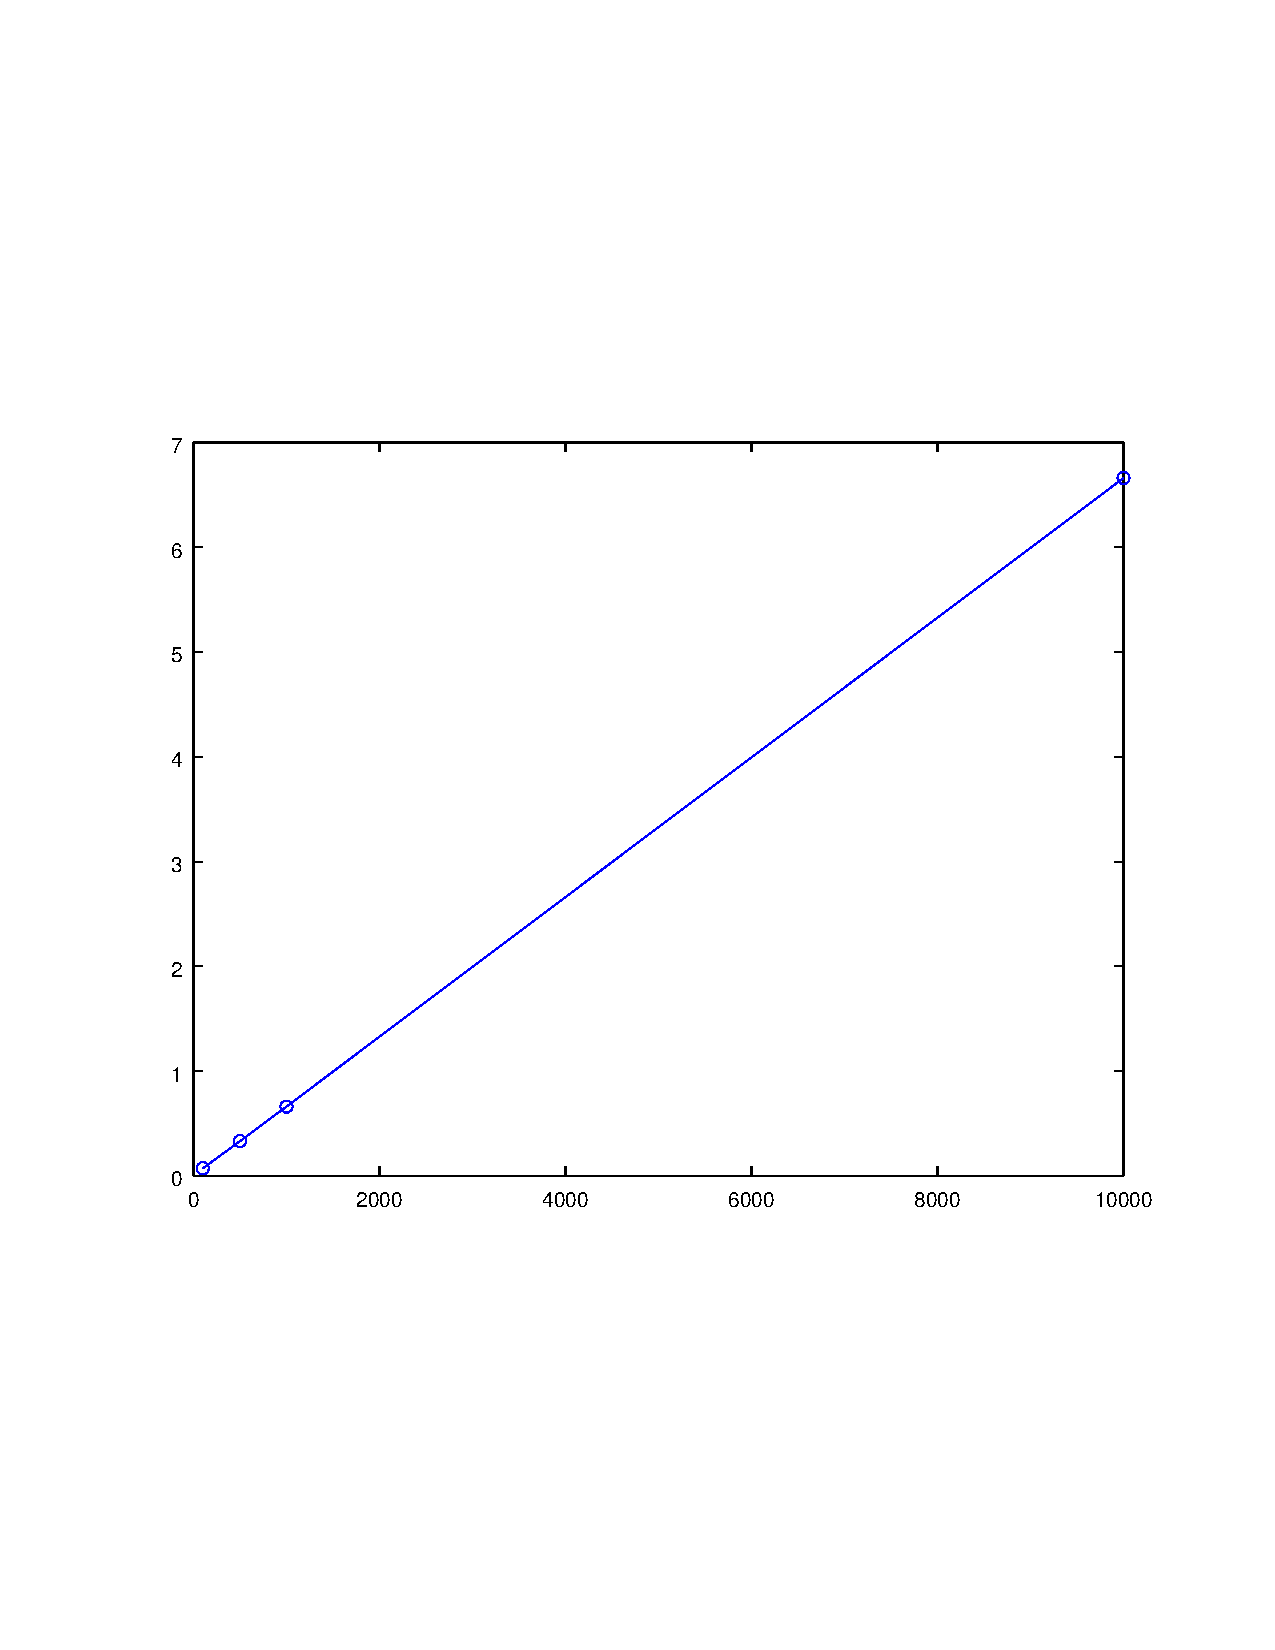
\includegraphics[height=\textheight]{Pics/lineartime1}
\end{center}
\end{frame}

\begin{frame}{Viðsnúningur strengs: Gerum betur}
Getum giskað á að \texttt{.join} aðgerðin taki langan tíma. Skrifum reverse-fall sem ekki notar það jafn oft:

\inputminted{python}{Code/Python/less_slow_reverse.py}

Athugum tímann á þessu falli líka.
\end{frame}

\begin{frame}{Prófanir}
Prófum að keyra \texttt{less\_slow\_reverse} við sömu aðstæður og hitt. Niðurstöður:

\begin{center}
\begin{tabular}{ll}
\toprule
$n$&$t_n$ (sek)\\
\midrule
100&0.012115\\
500&0.058038\\
1000&0.115067\\
10000&1.151805\\
\bottomrule
\end{tabular}
\end{center}

Miklu lægri tölur!
\end{frame}

\begin{frame}{Niðurstöður prófana - aftur bein lína}
\begin{center}
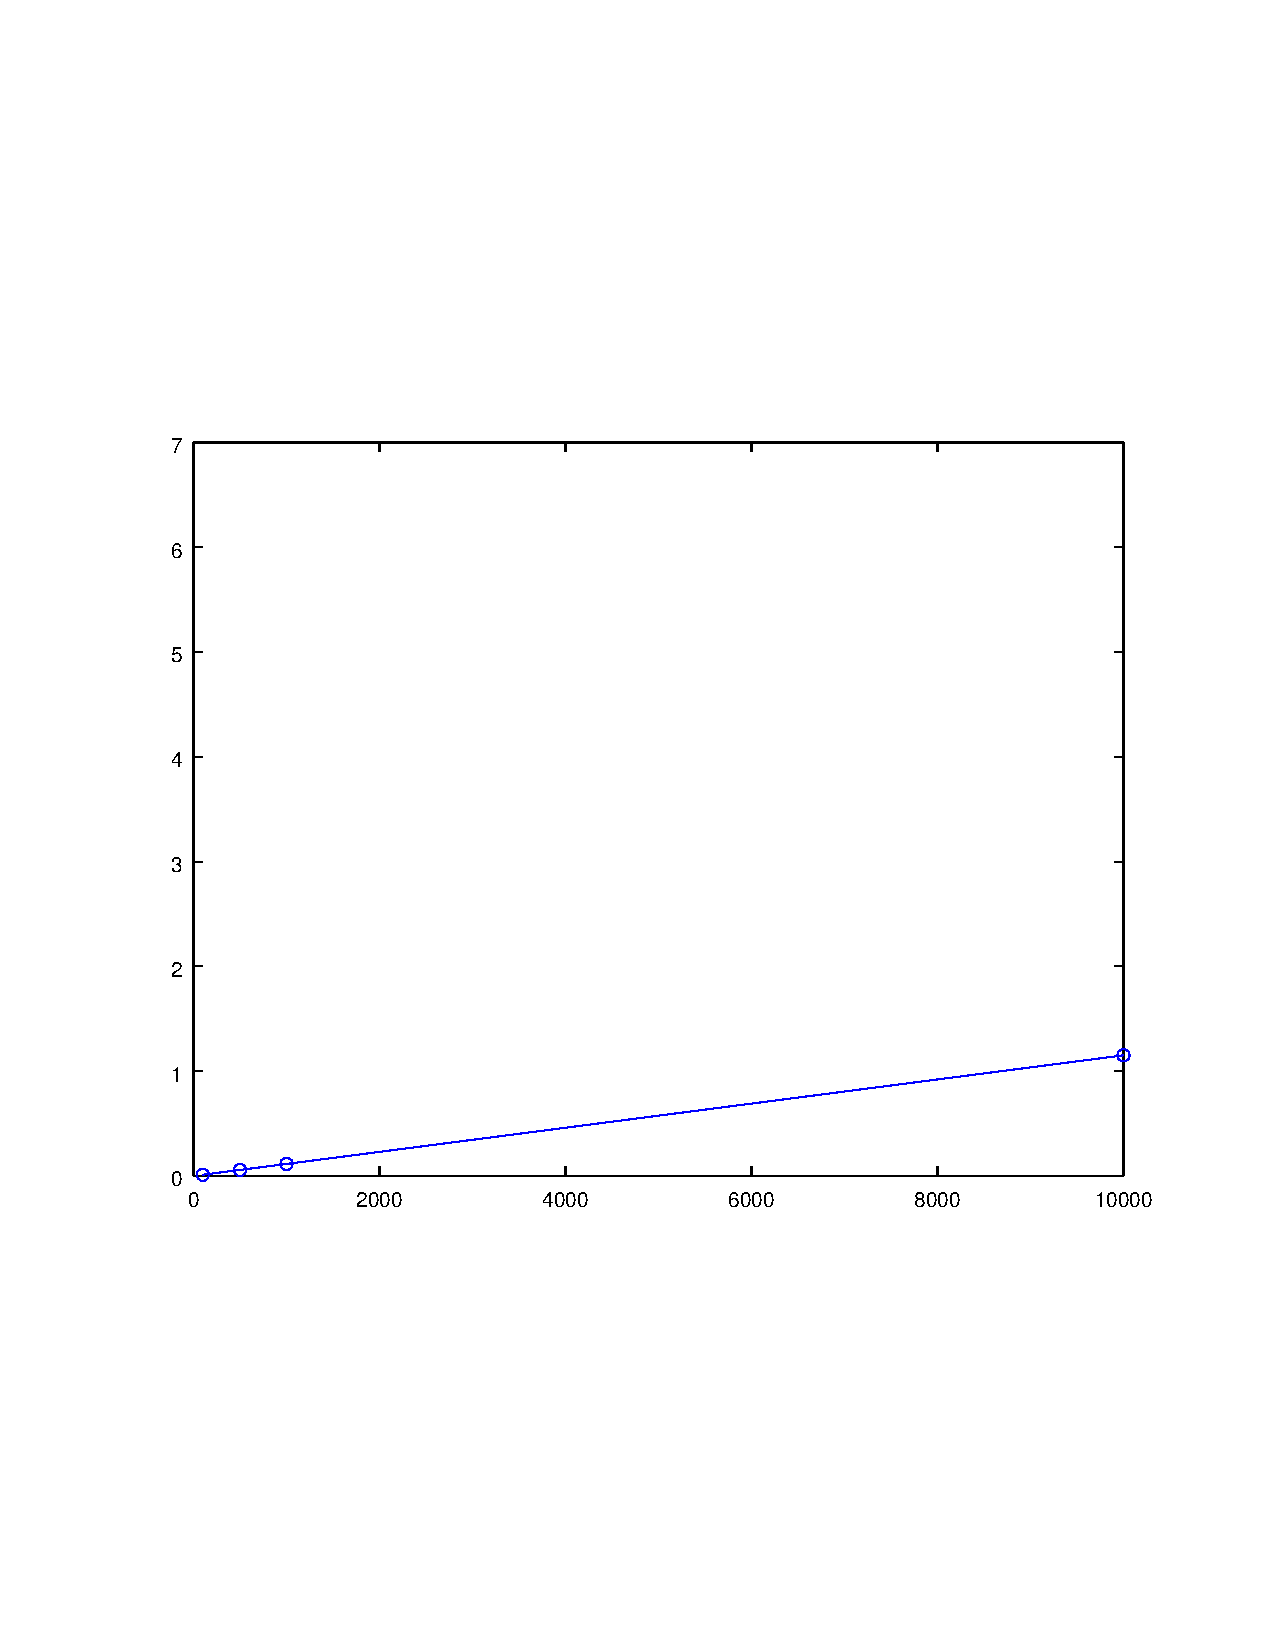
\includegraphics[height=\textheight]{Pics/lineartime2}
\end{center}
\end{frame}

\begin{frame}{Niðurstöður: Innbyggð aðferð}
Innbyggða leiðin \texttt{[::-1]} til að snúa við streng er mun hraðvirkari.

\begin{center}
\begin{tabular}{lll}
\toprule
$n$&$t_n$ (sek)&$\frac{(t_n - t_{n=1})\cdot10^7}{n}$\\
\midrule
100& 0.000211000&0.0000\\
500& 0.000551939&6.8187\\
1000& 0.001029015&8.1801\\
5000& 0.004233837&8.04567\\
10000& 0.008776903&8.5659\\
\bottomrule
\end{tabular}
\end{center}
Sjáum að þegar $n$ verður stórt vex $t_n$ nokkurn veginn í hlutfalli við lengd strengsins.
\end{frame}

\begin{frame}
\end{frame}

\end{document}